\documentclass[../piano_di_progetto.tex]{subfiles}

\begin{document}

La pianificazione si è basata sulle scadenze descritte nel sottocapitolo \S\ref{sub:scad}; il gruppo ha scelto di suddividere il periodo che va dalla formazione alla Revisione di Accettazione nelle seguenti fasi:
\begin{itemize}
\item \textbf{Analisi};
\item \textbf{Consolidamento dei requisiti};
\item \textbf{Progettazione e codifica della technology baseline};
\item \textbf{Progettazione e codifica di dettaglio};
\item \textbf{Validazione e collaudo}.
\end{itemize}
Ad ognuna di queste attività verranno destinate delle risorse di seguito descritte.

\subsection{Analisi}%
\label{sub:analisi}
Periodo: dal 2020-10-22 al 2021-01-10.\\
Questa attività si svolge nel periodo che va dalla formazione del gruppo alla consegna della \glossario{Revisione dei Requisiti}. In questo periodo il gruppo inizia con la visione dei \glossario{capitolati} proposti, e per ognuno di essi traccia un prototipo di \textsc{\glossario{studio di fattibilità}} dove vengono evidenziati gli aspetti positivi e negativi di ciascuno. Nel frattempo, vengono stabilite le prime \glossario{norme di progetto}, utili a fissare degli standard di utilizzo ai quali il gruppo si deve attenere. Successivamente alla scelta del capitolato vengono tracciati i requisiti minimi richiesti dal proponente, inoltre il gruppo incontra l'azienda tramite riunioni online allo scopo di risolvere eventuali dubbi.\\

\begin{figure}[H]
\centering
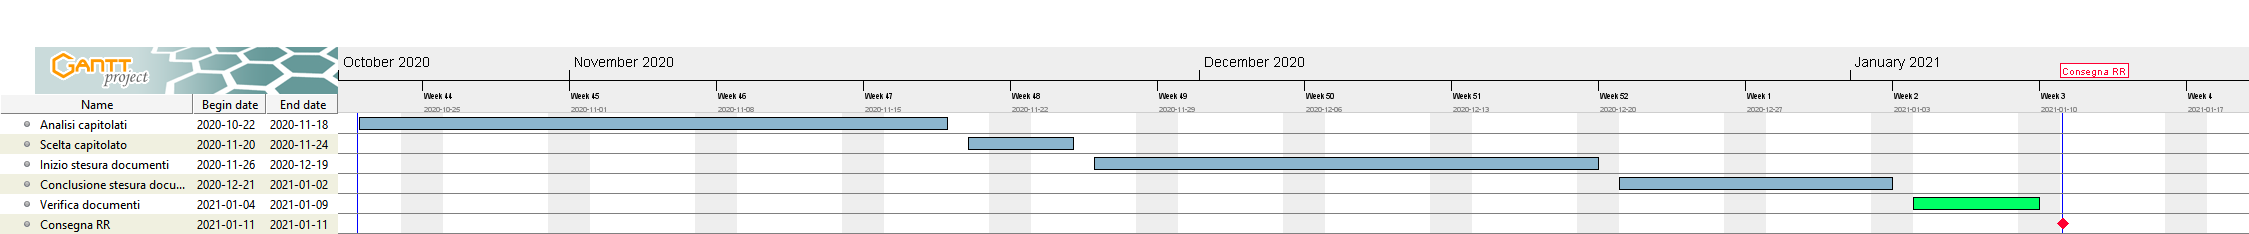
\includegraphics[width=18cm]{src/img/gantt/01_RR.png}
\caption{ \glossario{Diagramma di Gantt} della fase di analisi dei requisiti}

\end{figure}


\subsection{Consolidamento dei requisiti}%
\label{sub:cons_req}
Periodo: dal 11-01-2021 al 18-01-2021.\\
La fase di consolidamento dei requisiti inizia subito dopo la fase di analisi e finisce il giorno della presentazione della \textsc{Revisione dei Requisiti}.

\subsubsection*{Attività}
\begin{itemize}
    \item \textbf{Consolidamento}: attività che ha lo scopo di migliorare e/o consolidare i requisiti della fase precedente;
    \item \textbf{Preparazione della presentazione}: viene prodotto il materiale necessario all'esposizione che verrà esposta durante la RR;
    \item \textbf{Verifica documenti}: vengono verificati e, se necessario, aggiustati i documenti prodotti nelle fasi precedenti. 
\end{itemize}


%consegna della \textsc{Revisione dei Requisiti}; prevede l’approfondimento delle tecnologie richieste attraverso lo studio autonomo, l'approfondimento dell'analisi dei requisiti con eventuali aggiornamenti, se necessario. Sarà inoltre previsto qualche contatto con la \emph{Zucchetti S.p.A.} per fugare eventuali dubbi. Per concludere verrà preparata la presentazione. Questa fase si conclude con la presentazione della \textsc{Revisione dei Requisiti} giorno 18/01/2021.

\begin{figure}[H]
\centering
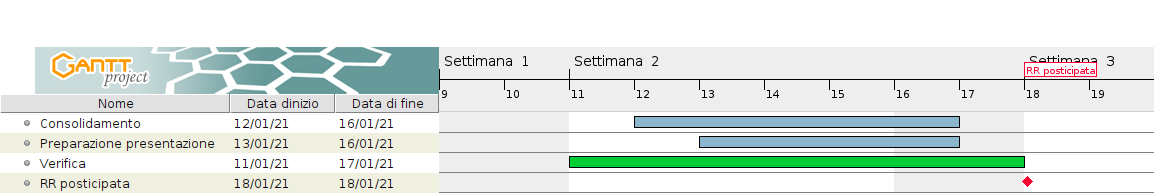
\includegraphics[width=18cm]{src/img/gantt/4_2_consolidamento_dei_requisiti.png}
\caption{ Diagramma di Gantt della fase di consolidamento dei requisiti}
\end{figure}


\subsection{Progettazione e codifica della technology baseline}
\label{sub:tech_baseline}
Periodo: dal 2021-01-19 al 2021-03-01. \\ \\
La fase di progettazione architetturale inizia subito dopo la presentazione della Revisione dei Requisiti.\\
In questa fase verranno aggiornati e corretti i documenti redatti a seguito delle valutazioni ricevute, saranno adattati i requisiti in base ai feedback del proponente e verrà effettuato uno studio più approfondito delle tecnologie coinvolte, al fine di realizzare un \glossario{Proof of Concept}.

\subsubsection*{Attività}
\begin{itemize}
    \item \textbf{Revisione/Aggiornamento}: revisione e/o aggiornamento di tutti i documenti \emph{v1.0.0} prodotti fino ad ora.
    \item \textbf{Ricerca tecnologie}: scelta di strumenti e tecnologie usate nella successiva fase di codifica del \glossario{Proof of Concept} previo studio autonomo;
    \item \textbf{Progettazione}: progettazione dell'architettura di sistema dell'applicazione;
    \item \textbf{Codifica}: codifica del Proof of Concept. 
    \item \textbf{Verifica}.\\
\end{itemize}
In questo periodo vengono scelti alcuni dei requisiti più rilevanti individuati durante la fase di Analisi e sviluppati in vari incrementi.
I requisti sono stati concordati con il proponente \textsc{Zucchetti S.p.A}, come dichiarato nel documento \textsc{Verbale Esterno 2021-02-17}.%

\subsection*{I incremento}
\textbf{Periodo (2021-01-19 - 2021-01-21)}\\
Vengono stabiliti i seguenti obiettivi:
\begin{itemize}
    \item Installazione e configurazione dell'ambiente di sviluppo Node.
\end{itemize}
\paragraph*{Attività}
\begin{itemize}
    \item Progettazione;
    \item Codifica;
    \item Verifica delle funzionalità implementate.
\end{itemize}

\subsection*{II incremento}
\textbf{Periodo (2021-01-22 - 2021-02-05)} \\
Vengono stabiliti i seguenti obiettivi:
\begin{itemize}
    \item Codifica del front-end dell'applicazione web \emph{HD Viz}.
\end{itemize}
\paragraph*{Attività}
\begin{itemize}
    \item Progettazione;
    \item Codifica;
    \item Verifica delle funzionalità implementate.
\end{itemize}

\subsection*{III incremento}
\textbf{Periodo (2021-01-25 - 2021-02-08)} \\
Vengono stabiliti i seguenti obiettivi:
\begin{itemize}
    \item Implementazione sistema di caricamento dati attraverso file CSV;
    \item Implementazione del parser dati e dell'assegnazione automatica delle label.
\end{itemize}
\paragraph*{Attività}
\begin{itemize}
    \item Progettazione;
    \item Codifica;
    \item Verifica delle funzionalità implementate.
\end{itemize}

\subsection*{IV incremento}
\textbf{Periodo (2021-02-09 - 2021-02-19)} \\
Vengono stabiliti i seguenti obiettivi:
\begin{itemize}
    \item Implementazione del grafico Scatter Plot Matrix per la visualizzazione dei dati importati.
\end{itemize}
\paragraph*{Attività}
\begin{itemize}
    \item Progettazione;
    \item Codifica;
    \item Verifica delle funzionalità implementate.
\end{itemize}

\subsubsection*{V incremento}
\textbf{Periodo (2021-02-12 - 2021-03-01)} \\
Vengono stabiliti i seguenti obiettivi:
\begin{itemize}
    \item Implementazione sistema di caricamento dati attraverso database.
\end{itemize}
\paragraph*{Attività}
\begin{itemize}
    \item Progettazione;
    \item Codifica;
    \item Lettera di presentazione;
    \item Consuntivo di periodo;
    \item Verifica delle funzionalità implementate.
\end{itemize}


\begin{figure}[H]
    \centering
    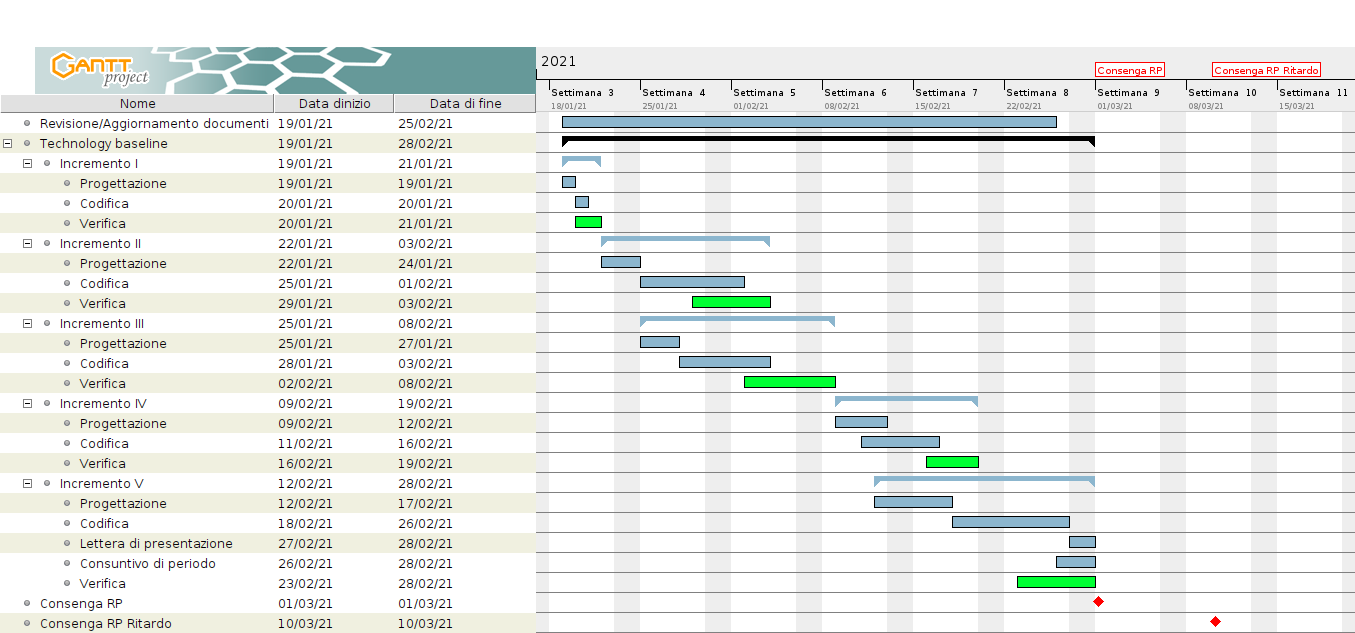
\includegraphics[width=18cm]{src/img/gantt/4_3_tech_baseline.png}
    \caption{Diagramma di Gantt della fase di progettazione della technology baseline}
\end{figure}


%===============================%

\subsection{Progettazione e codifica di dettaglio}%
\label{sub:prog_dett}

Periodo: dal 2021-03-10 al 2021-07-15.\\ \\
Inizialmente in questa fase si era previsto di proseguire il software realizzato in precedenza, tuttavia si è ritenuto opportuno ripartire da zero e realizzare prima un'architettura 
base che aiutasse successivamente nella programmazione. 
In questa fase si realizza la presentazione per la Revisione di Progettazione, stimata per giorno 2021-03-17, e si procede subito con la modifica di alcuni documenti quali
il \textsc{Piano di Progetto} per tracciare una prima pianificazione, e il \textsc{Piano di Qualifica} in quanto vi è necessità di iniziare a stilare obiettivi e metriche relativi al prodotto software.

Complessivamente questa fase è caratterizzata da due processi, quello di \emph{documentazione} e quello di \emph{progettazione e codifica}. Ad ogni incremento segue anche la rispettiva verifica. \\
Gli incrementi vengono assegnati a delle \emph{Milestones}, quindi il gruppo si da un tempo limite entro cui raggiungere determinati obiettivi e poi si ripianifica per la 
milestones successiva.\\
\textbf{Documenti:}
\begin{itemize}
    \item \textbf{Piano di progetto:}
        \begin{itemize}
            \item \textbf{Incremento I:} Si pianifica finemente la fase corrente, in quanto il tempo è poco e la successiva consegna è molto vicina;
            \item \textbf{Incremento II:} A ridosso della codifica del software si individuano gli incrementi da implementare;
            \item \textbf{Incremento III:} Si correggono eventuali errori segnalati tra gli esiti della Revisione di Progettazione;
            \item \textbf{Incremento IV:} Si realizza una nuova pianificazione;
            \item \textbf{Incremento V:} Si inviduano nuovi incrementi software;
            \item \textbf{Incremento IV:} Termine stesura;
        \end{itemize}
        \item \textbf{Piano di qualifica:}
        \begin{itemize}
            \item \textbf{Incremento I:} Si stilano le metriche e gli obiettivi relativi al prodotto software;
            \item \textbf{Incremento II:} Si correggono eventuali errori segnalati tra gli esiti della Revisione di Progettazione;
            \item \textbf{Incremento III:} Si aggiornano i capitoli relativi ai test svolti;
            \item \textbf{Incremento IV:} Termine stesura;
        \end{itemize}
        \item \textbf{Norme di progetto:}
        \begin{itemize}
            \item \textbf{Incremento I:} Si normano i diagrammi UML, i test che verranno effettuati, ed eventuali cambiamenti nell'amministrazione della repository;
            \item \textbf{Incremento II:} Si correggono eventuali errori segnalati tra gli esiti della Revisione di Progettazione;
        \end{itemize}
        \item \textbf{Manuale sviluppatore:}
        \begin{itemize}
            \item \textbf{Incremento I:} Si inizia la stesura generale del manuale sviluppatore;
            \item \textbf{Incremento II:} Aggiornamento del manuale;
            \item \textbf{Incremento III:} Ttermine stesura del manuale;
        \end{itemize}
        \item \textbf{Manuale utente:}
        \begin{itemize}
            \item \textbf{Incremento I:} Si inizia la stesura generale del manuale utente;
            \item \textbf{Incremento II:} Aggiornamento del manuale;
            \item \textbf{Incremento III:} Ttermine stesura del manuale;
        \end{itemize}
\end{itemize}

\textbf{HD-Viz:}
\begin{itemize}
    \item \textbf{Individuazione dell'architettura e creazione diagrammi:}
    \begin{itemize}
        \item \textbf{Incremento I:} Scelta del modello;
        \item \textbf{Incremento II:} Definizione dataset;
        \item \textbf{Incremento III:} Definizione grafici;
        \item \textbf{Incremento IV:} Definizione presenter e interfacce;
        \item \textbf{Incremento V:} Definizione view;
        \item \textbf{Incremento VI:} Definizione interazioni tra i tipi;      
    \end{itemize}

    \item \textbf{Correzione dell'architettura:}
    \begin{itemize}
        \item \textbf{Incremento I:} Si correggono le interazioni tra i tipi;
        \item \textbf{Incremento II:} Si corregge il server;
        \item \textbf{Incremento III:} Si aggiungono nuovi tipi;
    \end{itemize}

    \item \textbf{Codifica:}
    \begin{itemize}
    \item \textbf{Milestone 1:}
        \begin{itemize}
            \item \textbf{Incremento I:} Sviluppo ambiente di lavoro;
            \item \textbf{Incremento II:} Sviluppo inserimento dati tramite file;
            \item \textbf{Incremento III:} Sviluppo algoritmi di scelta;
    \end{itemize}

    \item \textbf{Milestone 2:}
        \begin{itemize}
            \item \textbf{Incremento IV:} Sviluppo Scatterplot Matrix;
            \item \textbf{Incremento V:} Sviluppo modifiche visualizzazioni;
	\end{itemize}
    \item \textbf{Milestone 3:}
        \begin{itemize}
            \item \textbf{Incremento VI:} Sviluppo visualizzazione errori;
            \item \textbf{Incremento VII:} Sviluppo modifiche DistanceMap;
            \item \textbf{Incremento VIII:} Sviluppo inserimento tramite database;
            \item \textbf{Incremento IX:} Estensione Scatterplot;
    \end{itemize}
    \item \textbf{Milestone 4:}
        \begin{itemize}
            \item \textbf{Incremento X:} Sviluppo modifica colori;
            \item \textbf{Incremento XI:} Sviluppo modifica dimensioni;
            \item \textbf{Incremento XII:} Sviluppo ForceField;
    \end{itemize}
    \item \textbf{Milestone 5:}
        \begin{itemize}
            \item \textbf{Incremento XIII:} Sviluppo PLMA;
            \item \textbf{Incremento XIV:} Sviluppo HeatMap;
    \end{itemize}
\end{itemize}
\end{itemize}


\begin{figure}[H]
    \centering
    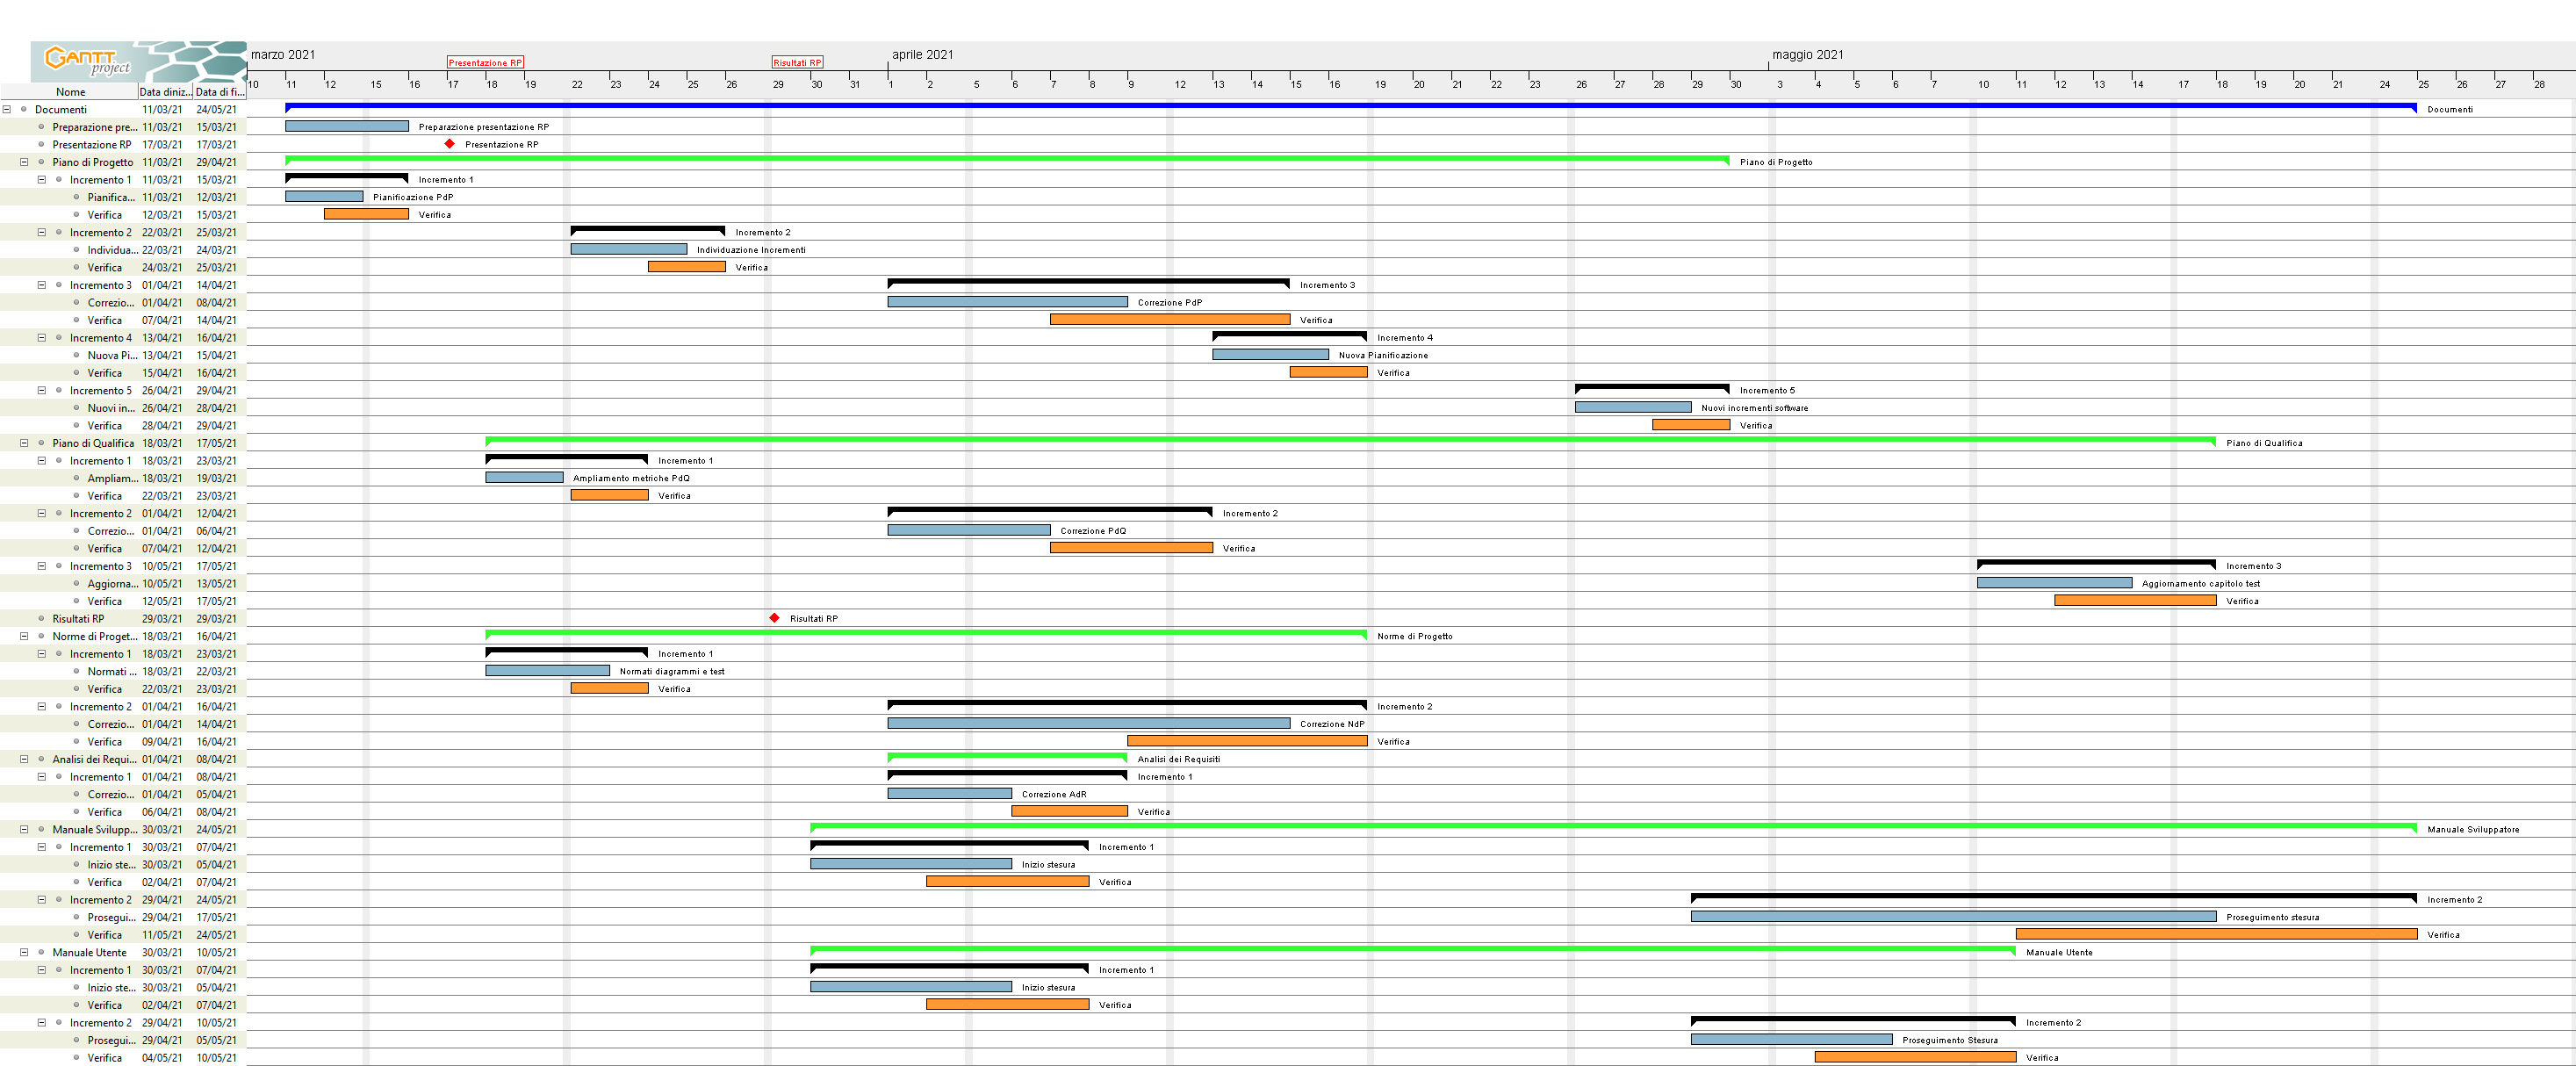
\includegraphics[width=18cm]{src/img/gantt/documenti_riveduti_RQ.png}
    \caption{Diagramma di Gantt della fase di progettazione e codifica}

\end{figure}

\begin{figure}[H]
    \centering
    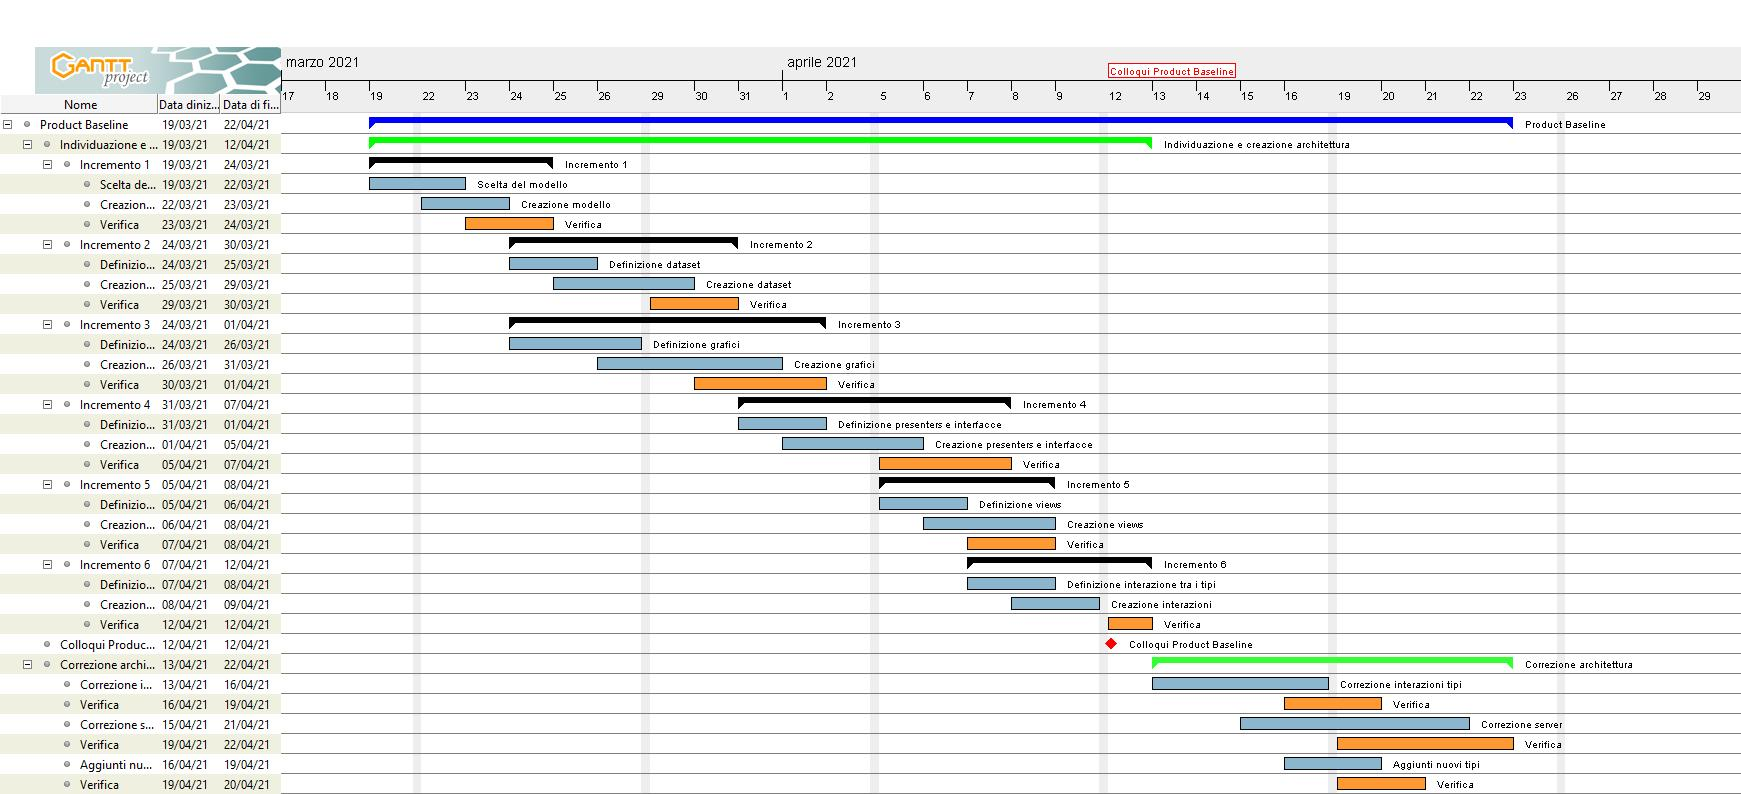
\includegraphics[width=18cm]{src/img/gantt/redazione_architettura_RQ.jpg}
    \caption{Diagramma di Gantt della fase di progettazione e codifica}

\end{figure}

\begin{figure}[H]
    \centering
    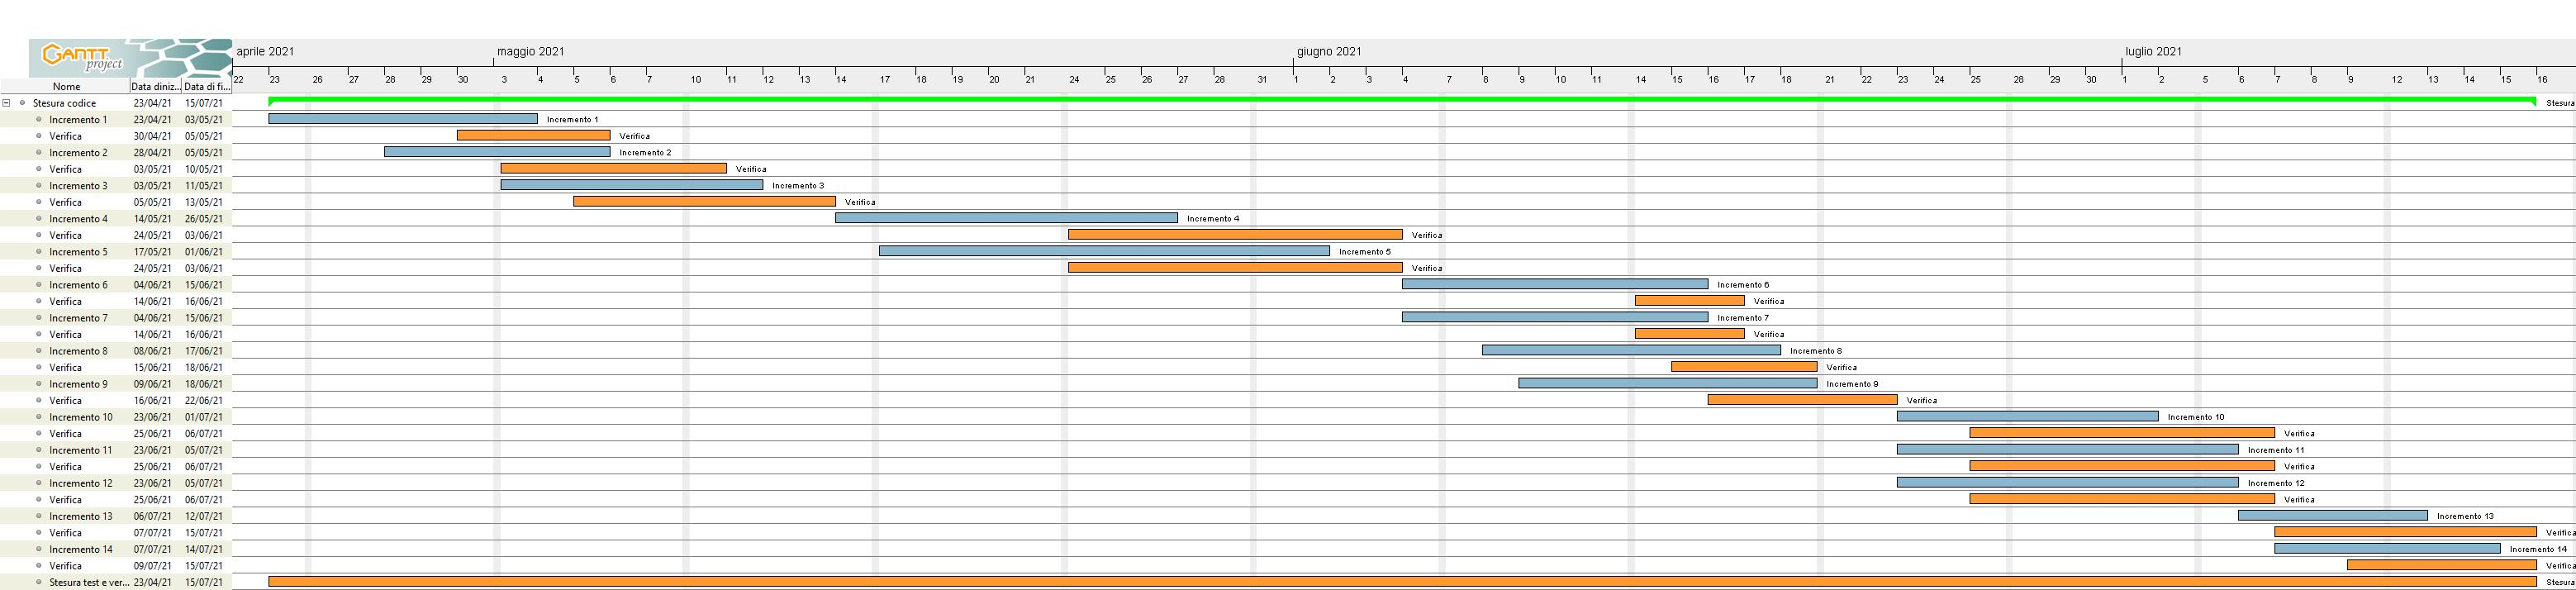
\includegraphics[width=18cm]{src/img/gantt/stesura_codiceRQ.jpg}
    \caption{Diagramma di Gantt della fase di progettazione e codifica}

\end{figure}

\begin{figure}[H]
    \centering
    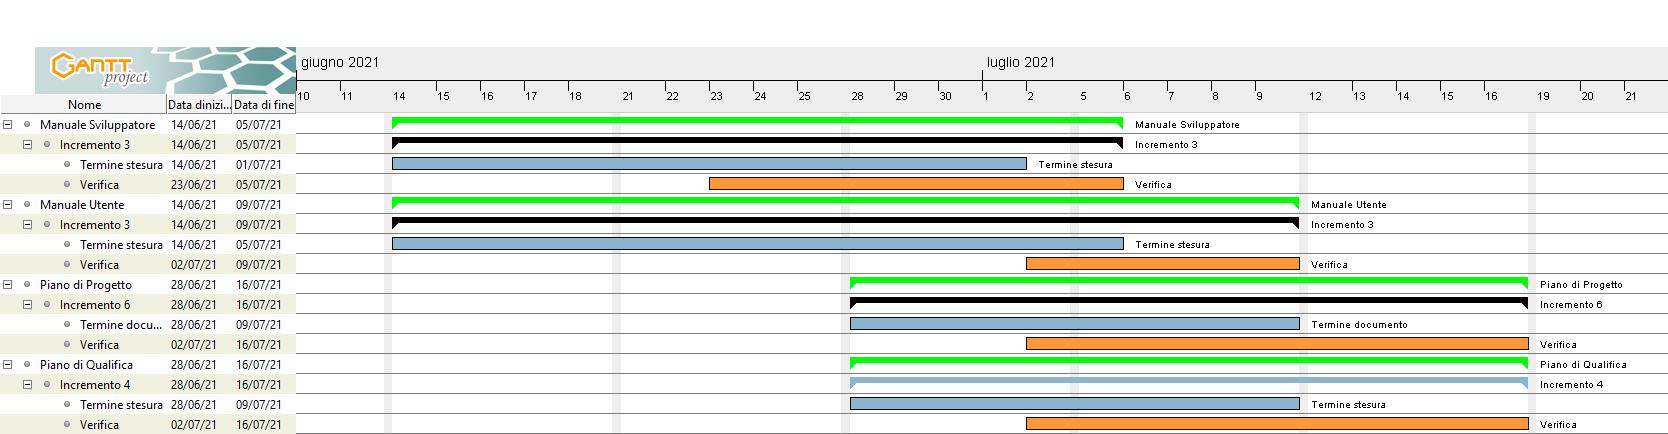
\includegraphics[width=18cm]{src/img/gantt/documenti_RQ_parte2.jpg}
    \caption{Diagramma di Gantt della fase di progettazione e codifica}
\end{figure}

%======================================%

\subsection{Validazione e Collaudo}%
\label{sub:valid_coll}
Periodo: 2021-07-16 al 2021-08-15 \\ \\ 
Questa fase terminerà con la \textsc{Revisione di Accettazione}. In questo periodo unico verranno svolte le seguenti attività:

\begin{itemize}
    \item Codifica: codifica della versione finale del prodotto, realizzando i requisiti opzionali rimanenti;
    \item Correzione e verifica dei documenti precedentemente redatti;
    \item Aggiornamento e verifica manuali: stesura della versione finale del \textsc{Manuale Utente} e \textsc{Manuale Sviluppatore};
    \item Validazione: verifica di conformità rispetto agli obiettivi;
    \item Collaudo: test di collaudo per ogni funzionalità del prodotto;
    \item Preparazione presentazione.
\end{itemize}

Per quanto riguarda la produzione software sono previsti i seguenti incrementi:
\begin{itemize}
    \item \textbf{Incremento XV:} sviluppo requisiti rimanendi Scatterplot;
    \item \textbf{Incremento XVI:} sviluppo requisiti rimanendi ForceField - parte 1;
    \item \textbf{Incremento XVII:} sviluppo requisiti rimanendi ForceField - parte 2;
    \item \textbf{Incremento XVIII:} sviluppo requisiti HeatMap;
    \item \textbf{Incremento XIX:} sviluppo requisiti DistanceMap;
    \item \textbf{Incremento XX:} requisiti rimanenti;
\end{itemize}


\begin{figure}[H]
\centering
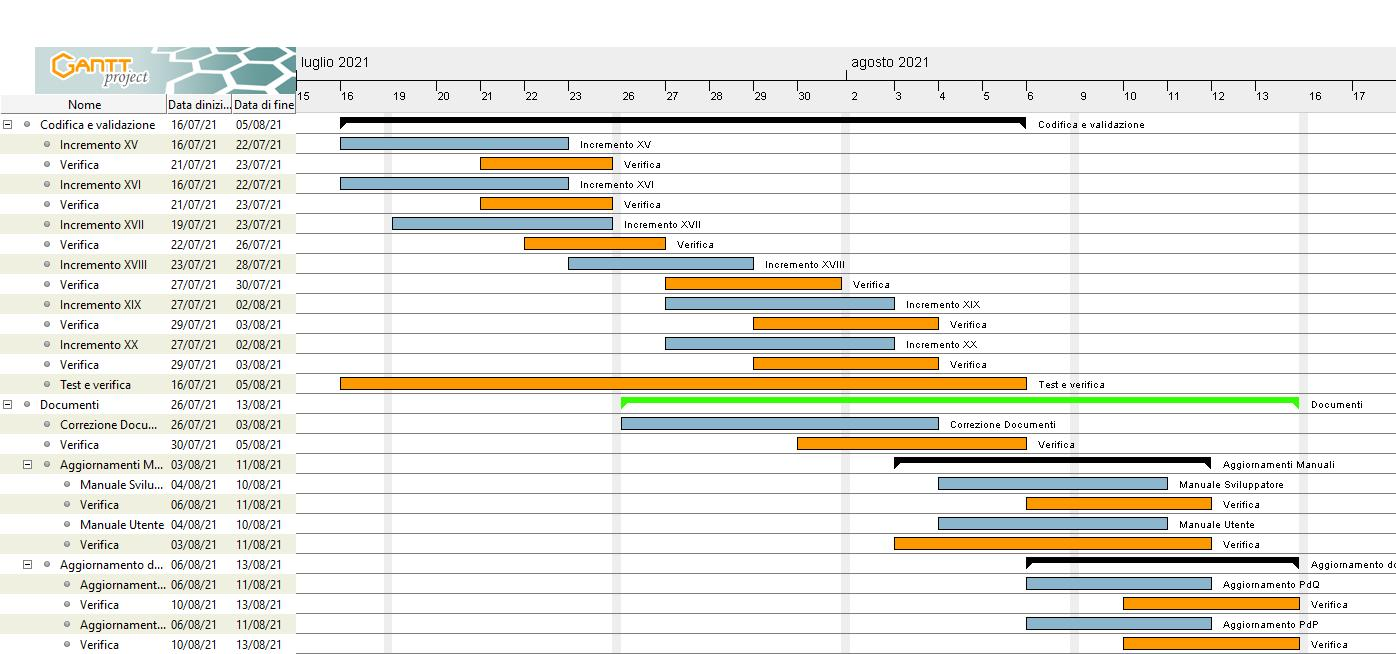
\includegraphics[width=18cm]{src/img/gantt/pianif_RA.jpg}
\caption{Diagramma di Gantt della fase di validazione e collaudo}
\end{figure}

\end{document}
